% -*- LaTeX -*-
% -*- coding: utf-8 -*-
%
% ~~~~~~~~~~~~~~~~~~~~~~~~~~~~~~~~~~~~~~~~~~~~~~~~~~~~~~~~~~~~~~~~~~~~~~~~~~~~~~
%
%                             michael a.g. aïvázis
%                      california institute of technology
%                      (c) 1998-2010  all rights reserved
%
% ~~~~~~~~~~~~~~~~~~~~~~~~~~~~~~~~~~~~~~~~~~~~~~~~~~~~~~~~~~~~~~~~~~~~~~~~~~~~~~
%

\lecture{Programming with pthreads}{20100120}

% --------------------------------------
% threads and shared memory parallelism 
\begin{frame}[fragile]
%
  \frametitle{Threads and shared memory parallelism}
%
  \begin{itemize}
%
  \item recall the shared memory architecture
%
    \begin{figure}
      \centering
      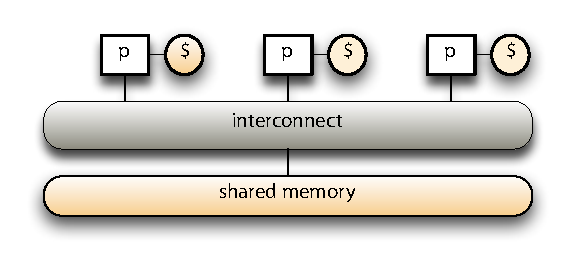
\includegraphics[scale=0.5]{figures/shared-memory.pdf}
    \end{figure}
    \vspace{-1.0em}
%
    \begin{itemize}
    \item processors are connected to a memory pool with a global address space
    \item processors have their own cache but no private memory
    \end{itemize}
%
  \item model is relevant for {\em threads}
%
    \begin{itemize}
    \item lightweight processes that can be scheduled independently, but share many OS
      resources
      \begin{itemize}
      \item CPU
      \item memory
      \item but also file descriptors, process environment, etc.
      \end{itemize}
    \item supported by most modern operating systems
    \end{itemize}
%
  \end{itemize}
%
    \begin{figure}
      \centering
      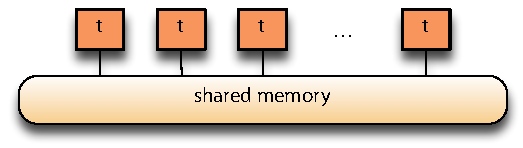
\includegraphics[scale=0.5]{figures/threads-memory.pdf}
    \end{figure}
%
\end{frame}

% --------------------------------------
% template
\begin{frame}[fragile]
%
  \frametitle{Processes and threads}
%
  \begin{itemize}
%
  \item in most operating systems, a process has
    \begin{itemize}
    \item process id and group id, user id and group id
    \item environment variables
    \item working directory
    \item scheduling information
    \item registers, stack, heap, instruction stream
    \item file descriptors, signal handlers, other process dependent structures
    \end{itemize}
%
  \item threads 
    \begin{itemize}
      \item share many of the per-process properties
        \begin{itemize}
        \item they are lightweight since they incur low overhead
        \end{itemize}
      \item have their own copy of
        \begin{itemize}
        \item registers, stack, instruction stream
        \item scheduling information
        \end{itemize}
    \end{itemize}
%
  \item threads are important programming constructs
    \begin{itemize}
    \item every vendor supports a proprietary interface
    \item {\em pthreads}, the POSIX standard API specification brought portability
    \item standardized creation, management, synchronization
    \end{itemize}
%
  \end{itemize}
%
\end{frame}

% --------------------------------------
% template
\begin{frame}[fragile]
%
  \frametitle{The pthreads API}
%
  \begin{itemize}
%
  \item threads require support from the compiler, the linker, the loader, and the OS kernel
    \begin{itemize}
    \item thread safety
    \end{itemize}
%
  \item special command line argument to most compliant compilers
    \begin{itemize}
    \item changes the instruction strategy
    \item adds the pthread runtime library to the link line
    \item links against the thread safe runtime
    \end{itemize}
%
  \item naming conventions
    \begin{table}
      \scriptsize
      \centering
      \begin{tabular}{l|l}
        Prefix & Functional group\\ \hline
        {\tt pthread\_ } &
            access to the threads, and some miscellaneous routines\\
        {\tt pthread\_attr\_ } & 
            thread attribute objects\\
        {\tt pthread\_mutex\_ } & 
            mutexes\\
        {\tt pthread\_mutexattr\_ } & 
            mutex attribute objects\\
        {\tt pthread\_cond\_ } & 
            condition variables\\
        {\tt pthread\_condattr\_ } & 
            condition variable attribute objects\\
        {\tt pthread\_key\_ } & 
            thread-specific data keys\\
        {\tt pthread\_rwlock\_ } & 
            read/write locks\\
        {\tt pthread\_barrier\_ } & 
            synchronization barriers\\
      \end{tabular}
    \end{table}
%
  \item the standard specifies the API for \CC\ only; \fortran\ support varies
    \begin{itemize}
    \item must include \srcfile{pthread.h}
    \end{itemize}
%
  \item lots of good books; see \href{http://acm114.caltech.edu/references}
%
  \end{itemize}
%
\end{frame}

% --------------------------------------
% template
\begin{frame}[fragile]
%
  \frametitle{Creating threads}
  \begin{itemize}
%
  \item create threads by calling
%
  \begin{C}
int pthread_create(
    pthread_t* id, const pthread_attr_t* attr,
    void* (*startup)(void*), void* arg);
  \end{C}
%
\item initially a process has one thread; every other thread must be explicitly created
  by calling \function{pthread\_create} and passing
  \begin{itemize}
  \item \identifier{id}: the location where a unique thread identifier will be stored
  \item \identifier{attr}: an opaque attribute object with thread initialization options
  \item \function{startup}: a pointer to a \CC\ function that will be executed by the thread
    once it gets scheduled
  \item \identifier{arg}: user defined data to be passed to \function{startup}; may be \NULL
  \end{itemize}
%
  \item once scheduled, threads are first class citizens
%
  \item the maximum number of threads per process depends on the implementation
%
  \end{itemize}
%
    \begin{figure}
      \centering
      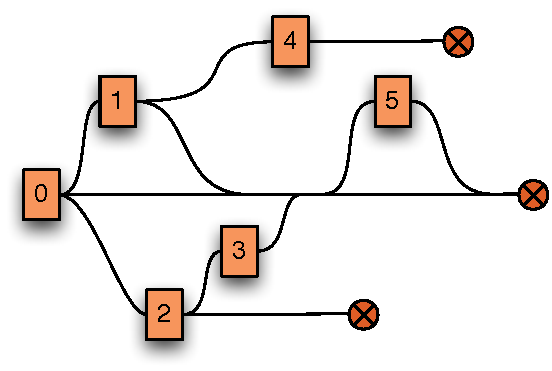
\includegraphics[scale=0.5]{figures/threads.pdf}
    \end{figure}
%
\end{frame}

% --------------------------------------
% terminating threads
\begin{frame}[fragile]
%
  \frametitle{Terminating threads}
%
  \begin{itemize}
%
    \item several ways to terminate a thread
      \begin{itemize}
      \item the thread returns from \function{main}
      \item the thread explicitly calls \function{pthread\_exit}
      \item the thread is killed when another thread calls \function{pthread\_cancel}
      \item the process terminates due to some system call, e.g.~\function{exit},
        \function{exec}, etc.
      \end{itemize}
%
  \item use \function{pthread\_exit} to kill a thread when it is no longer needed
%
    \begin{C}
int pthread_exit(void * status);
    \end{C}
%
  \item if \function{main} finishes and any threads remain
    \begin{itemize}
    \item they get killed unless \function{main} has called \function{pthread\_exit}
    \item otherwise they continue to run
    \end{itemize}
%
  \item thread routines do not have to call \function{pthread\_exit} unless they intend to pass
    their termination status to their creator
%
  \item \function{pthread\_exit} does not perform any process cleanup: it doesn't flush/close
    files, release other resources, signal the process parent, etc.
  \end{itemize}
%
\end{frame}

% --------------------------------------
% hello world
\begin{frame}[fragile]
%
  \frametitle{Hello world}
%
  \begin{C}
#include <pthread.h>
#include <stdio.h>
#define THREADS 10

void* hello(void* threadID) {
    long id = (long) threadID;
    printf("hello from %02ld/%0d\n", id, THREADS);
    pthread_exit(NULL);
    return NULL;
}

int main(int argc, char* argv[]) {
    long id;
    int status;
    pthread_t threads[THREADS];

    for (id=0; id<THREADS; id++) {
        printf("creating thread %02ld\n", id);
        status = pthread_create(&threads[id], NULL, hello, (void*) id);
        if (status) {
            printf("error %d in pthread_create\n", status);
        }
    }
    /* there is a problem here... */
    pthread_exit(NULL);
    return 0;
}
  \end{C}
%
\end{frame}

% end of file 
